\documentclass[12pt,tikz,border=4mm]{standalone}

\usepackage{fontspec}
\usepackage{xeCJK}
\usepackage{xcolor}
\usetikzlibrary{arrows.meta,backgrounds,calc,fit,positioning}

\setsansfont{Noto Sans CJK SC}
\setCJKsansfont{Noto Sans CJK SC}
\renewcommand{\familydefault}{\sfdefault}

\definecolor{signal}{HTML}{009E73}
\definecolor{prompt}{HTML}{0072B2}
\definecolor{delayed}{HTML}{D55E00}
\definecolor{shared}{HTML}{4E5D6C}
\definecolor{ink}{HTML}{1F2933}

\begin{document}
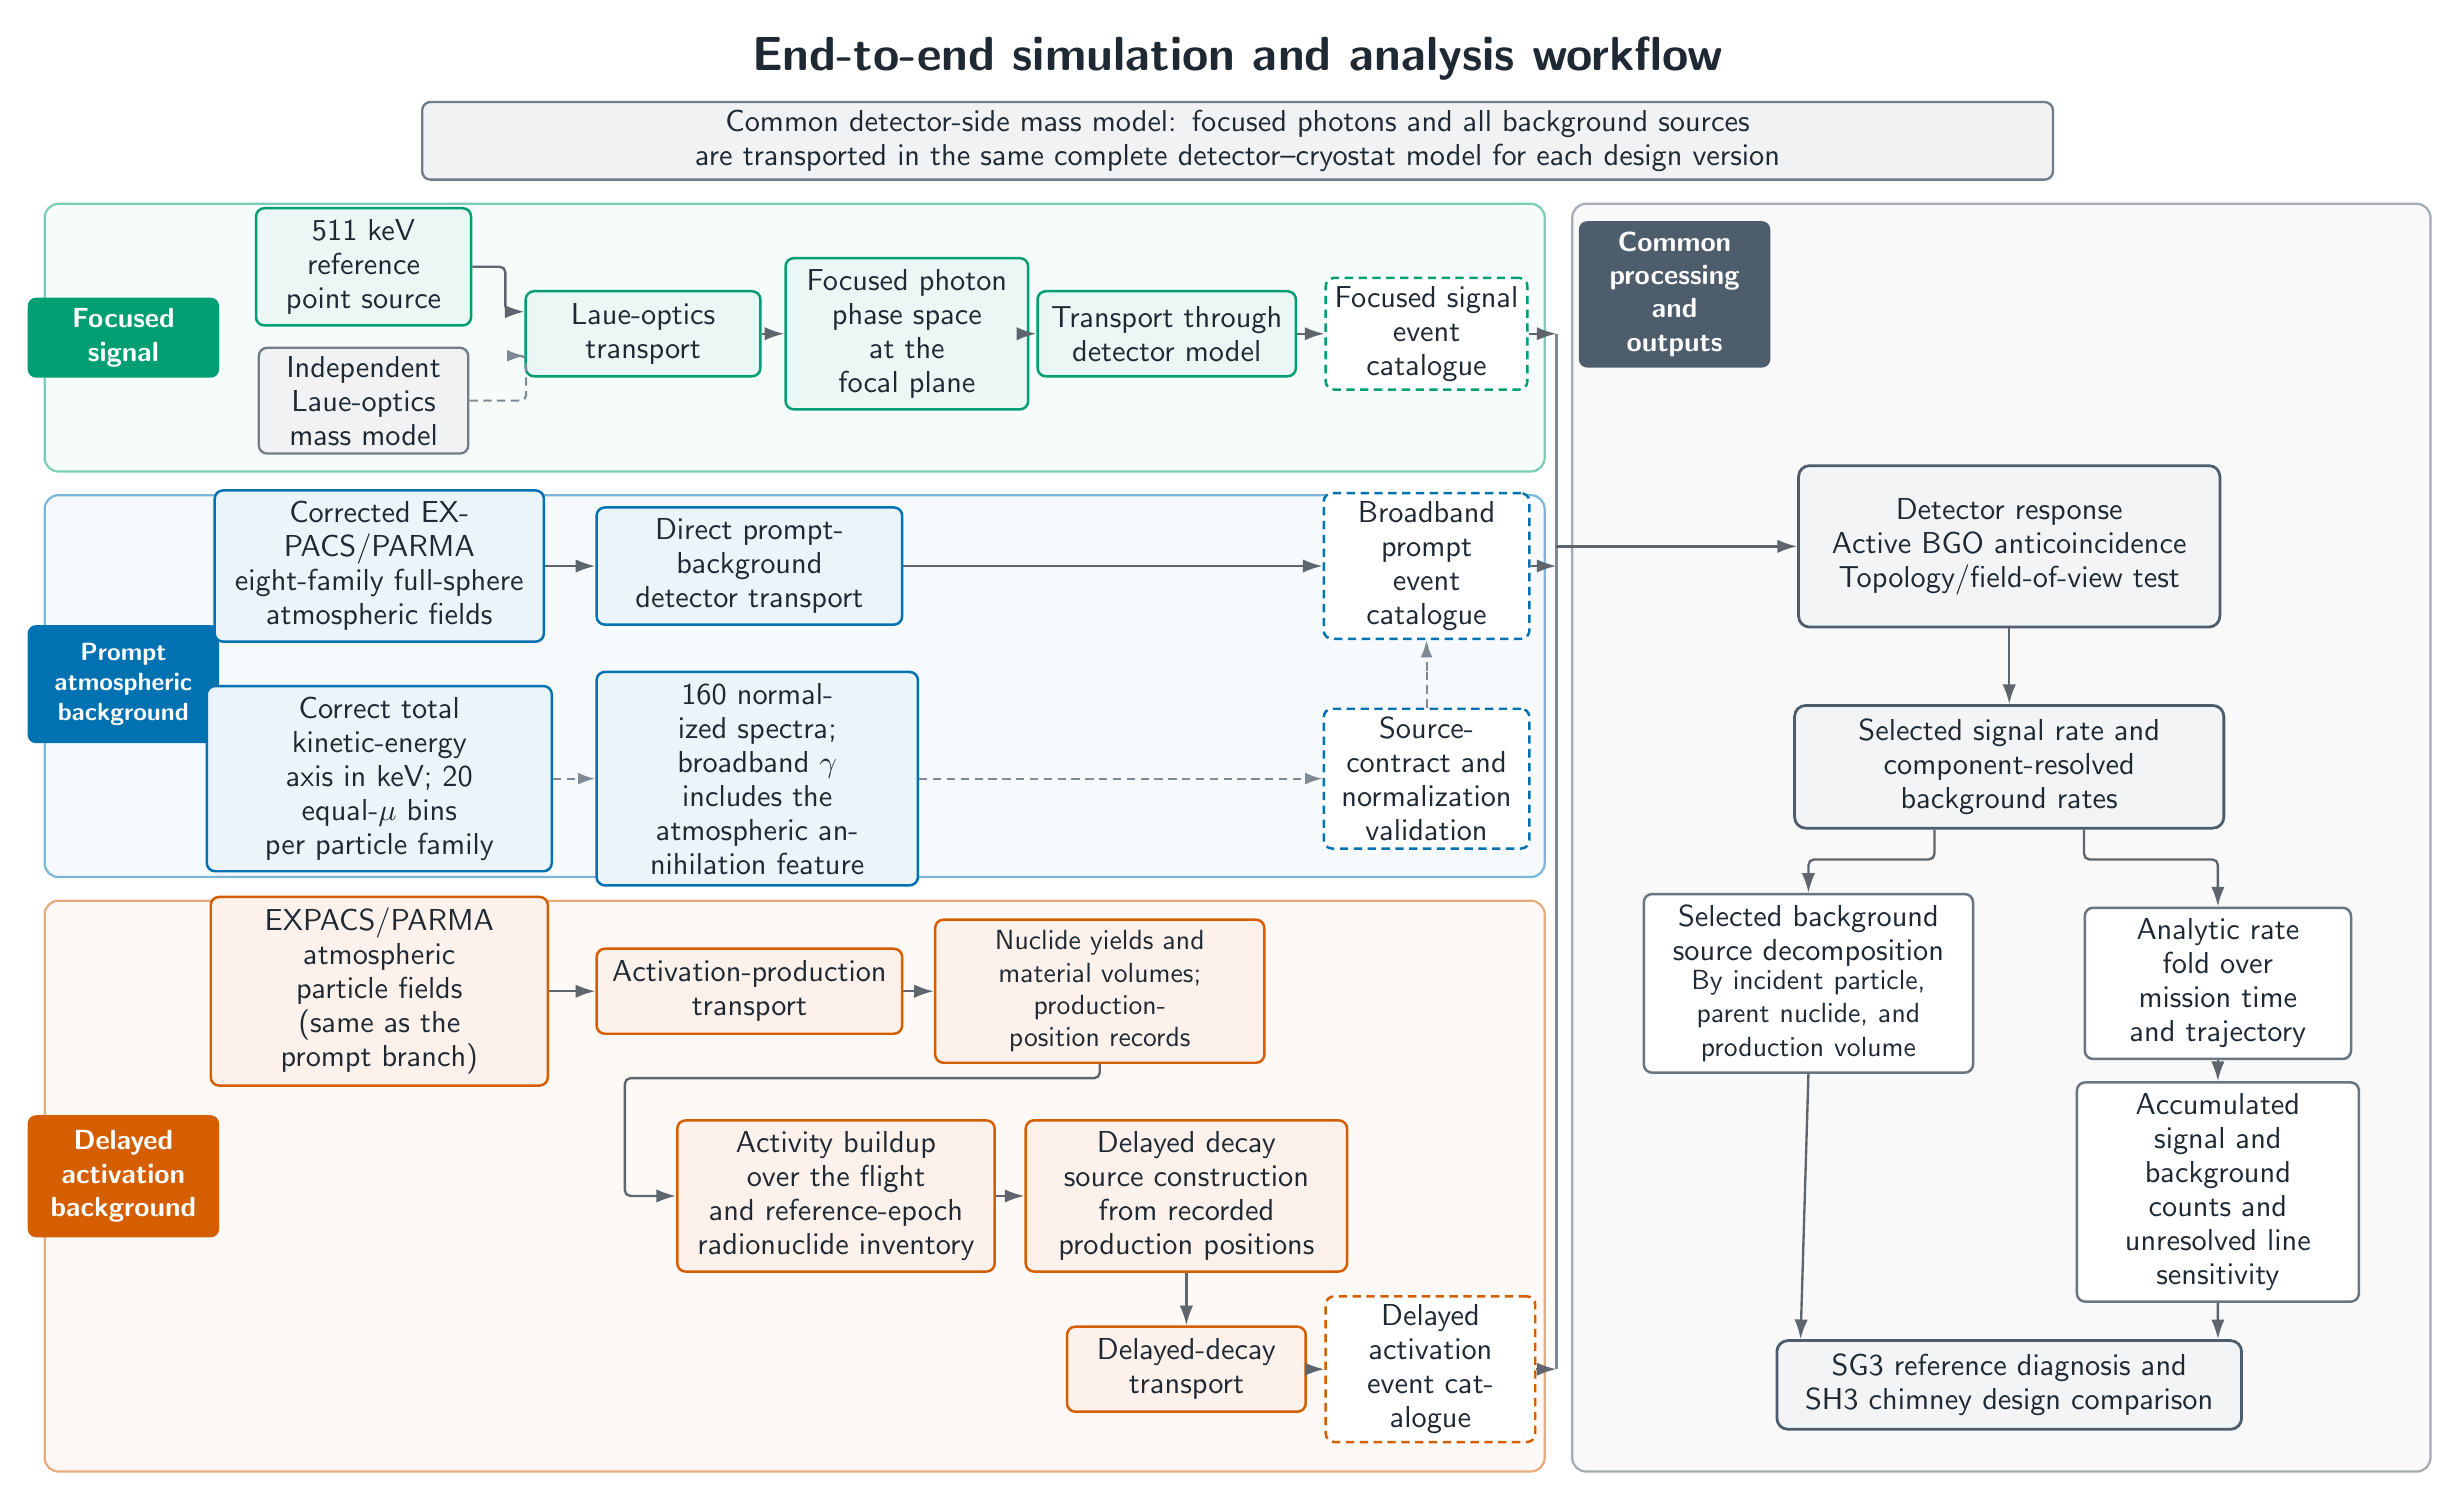
\begin{tikzpicture}[
  x=1cm,
  y=1cm,
  text=ink,
  font=\fontsize{10.6pt}{12.3pt}\selectfont,
  flow/.style={-{Latex[length=2.5mm,width=1.7mm]}, draw=ink!72,
               line width=0.85pt, rounded corners=2pt},
  dep/.style={-{Latex[length=2.2mm,width=1.5mm]}, draw=shared!72,
              line width=0.75pt, densely dashed, rounded corners=2pt},
  signalbox/.style={rectangle, rounded corners=3pt, draw=signal,
                   fill=signal!8, line width=0.9pt, align=center,
                   text width=2.55cm, minimum height=1.08cm, inner sep=4pt},
  promptbox/.style={rectangle, rounded corners=3pt, draw=prompt,
                   fill=prompt!8, line width=0.9pt, align=center,
                   text width=2.95cm, minimum height=1.08cm, inner sep=4pt},
  delayedbox/.style={rectangle, rounded corners=3pt, draw=delayed,
                    fill=delayed!8, line width=0.9pt, align=center,
                    text width=2.75cm, minimum height=1.08cm, inner sep=4pt},
  modelbox/.style={rectangle, rounded corners=3pt, draw=shared!80,
                  fill=shared!8, line width=0.85pt, align=center,
                  text width=2.7cm, minimum height=0.9cm, inner sep=3pt},
  eventbox/.style={rectangle, rounded corners=3pt, draw=#1,
                  fill=white, densely dashed, line width=0.9pt, align=center,
                  text width=2.25cm, minimum height=0.92cm, inner sep=3pt},
  sharedbox/.style={rectangle, rounded corners=4pt, draw=shared,
                   fill=shared!7, line width=1.0pt, align=center,
                   text width=4.65cm, minimum height=1.08cm, inner sep=5pt},
  outputbox/.style={rectangle, rounded corners=3pt, draw=shared!85,
                   fill=white, line width=0.9pt, align=center,
                   text width=2.35cm, minimum height=1.0cm, inner sep=4pt},
  lanehead/.style={rounded corners=3pt, text=white, align=center,
                  font=\fontsize{10.3pt}{12pt}\selectfont\bfseries,
                  text width=2.15cm, minimum width=2.35cm,
                  minimum height=1.0cm, inner sep=4pt},
  smallnote/.style={font=\fontsize{9.7pt}{11.3pt}\selectfont,
                   text=ink!82, align=left}
]

% Title and shared detector-model contract
\node[font=\fontsize{16pt}{18pt}\selectfont\bfseries, text=ink]
  at (15.30,1.2) {End-to-end simulation and analysis workflow};

\node[modelbox, text width=20.5cm, minimum height=0.76cm] (detmodel)
  at (15.30,0.15)
  {Common detector-side mass model: focused photons and all background sources\\are transported in the same complete detector--cryostat model for each design version};

% Lane backgrounds
\begin{scope}[on background layer]
  \filldraw[rounded corners=5pt, fill=signal!3.5, draw=signal!52, line width=0.8pt]
    (0.15,-0.65) rectangle (19.20,-4.05);
  \filldraw[rounded corners=5pt, fill=prompt!3.5, draw=prompt!52, line width=0.8pt]
    (0.15,-4.35) rectangle (19.20,-9.20);
  \filldraw[rounded corners=5pt, fill=delayed!3.5, draw=delayed!52, line width=0.8pt]
    (0.15,-9.50) rectangle (19.20,-16.75);
  \filldraw[rounded corners=5pt, fill=shared!3.5, draw=shared!52, line width=0.8pt]
    (19.55,-0.65) rectangle (30.45,-16.75);
\end{scope}

% Lane labels
\node[lanehead, fill=signal] at (1.15,-2.35) {Focused signal};
\node[lanehead, fill=prompt, minimum height=1.50cm,
      font=\fontsize{9.4pt}{10.8pt}\selectfont\bfseries] at (1.15,-6.75)
  {Prompt\\atmospheric\\background};
\node[lanehead, fill=delayed, minimum height=1.55cm] at (1.15,-13.00)
  {Delayed activation\\background};
\node[lanehead, fill=shared, minimum height=1.55cm] at (20.85,-1.80)
  {Common\\processing\\and\\outputs};

% Focused-signal lane
\node[signalbox, text width=2.45cm] (src) at (4.20,-1.45)
  {511 keV reference\\point source};
\node[modelbox, text width=2.45cm] (optmodel) at (4.20,-3.15)
  {Independent Laue-optics\\mass model};
\node[signalbox, text width=2.70cm] (optics) at (7.75,-2.30)
  {Laue-optics transport};
\node[signalbox, text width=2.80cm] (phase) at (11.10,-2.30)
  {Focused photon\\phase space at the\\focal plane};
\node[signalbox, text width=3.00cm] (dettransport) at (14.40,-2.30)
  {Transport through\\detector model};
\node[eventbox=signal, text width=2.35cm] (sigevt) at (17.70,-2.30)
  {Focused signal\\event catalogue};

\draw[flow] (src.east) -- ++(0.42,0) |- ($(optics.west)+(0,0.28)$);
\draw[dep] (optmodel.east) -- ++(0.72,0) |- ($(optics.west)+(0,-0.28)$);
\draw[flow] (optics) -- (phase);
\draw[flow] (phase) -- (dettransport);
\draw[flow] (dettransport) -- (sigevt);

% Prompt-background lane: current corrected source and its contract validation
\node[promptbox, text width=3.90cm] (expacs) at (4.40,-5.25)
  {Corrected EXPACS/PARMA\\eight-family full-sphere\\atmospheric fields};
\node[promptbox, text width=3.60cm] (prompttr) at (9.10,-5.25)
  {Direct prompt-background\\detector transport};
\node[eventbox=prompt, text width=2.40cm] (promptevt) at (17.70,-5.25)
  {Broadband prompt\\event catalogue};

\node[promptbox, text width=4.10cm] (linesrc) at (4.40,-7.95)
  {Correct total kinetic-energy\\axis in keV; 20 equal-$\mu$ bins\\per particle family};
\node[promptbox, text width=3.80cm] (linetr) at (9.20,-7.95)
  {160 normalized spectra;\\broadband $\gamma$ includes the\\atmospheric annihilation feature};
\node[eventbox=prompt, text width=2.40cm] (lineevt) at (17.70,-7.95)
  {Source-contract and\\normalization validation};

\draw[flow] (expacs) -- (prompttr);
\draw[flow] (prompttr) -- (promptevt);
\draw[dep] (linesrc) -- (linetr);
\draw[dep] (linetr) -- (lineevt);
\draw[dep] (lineevt.north) -- ++(0,0.42) -| (promptevt.south);

% Delayed-activation lane: independent BUILDUP chain
\node[delayedbox, text width=4.00cm] (expacs2) at (4.40,-10.65)
  {EXPACS/PARMA\\atmospheric particle fields\\(same as the prompt branch)};
\node[delayedbox, text width=3.60cm] (buildup) at (9.10,-10.65)
  {Activation-production\\transport};
\node[delayedbox, text width=3.90cm,
      font=\fontsize{10pt}{11.6pt}\selectfont] (records) at (13.55,-10.65)
  {Nuclide yields and\\material volumes;\\production-position records};

\node[delayedbox, text width=3.75cm] (inventory) at (10.20,-13.25)
  {Activity buildup over the flight\\and reference-epoch\\radionuclide inventory};
\node[delayedbox, text width=3.80cm] (dsrc) at (14.65,-13.25)
  {Delayed decay\\source construction\\from recorded\\production positions};
\node[delayedbox, text width=2.75cm] (decaytr) at (14.65,-15.45)
  {Delayed-decay transport};
\node[eventbox=delayed, text width=2.45cm] (delayevt) at (17.75,-15.45)
  {Delayed activation\\event catalogue};

\draw[flow] (expacs2) -- (buildup);
\draw[flow] (buildup) -- (records);
\coordinate (inventoryRouteA) at ($(records.south)+(0,-0.18)$);
\coordinate (inventoryRouteB) at ($(inventory.west)+(-0.65,0)$);
\draw[flow] (records.south) -- (inventoryRouteA)
  -| (inventoryRouteB) -- (inventory.west);
\draw[flow] (inventory) -- (dsrc);
\draw[flow] (dsrc) -- (decaytr);
\draw[flow] (decaytr) -- (delayevt);

% Event-stream bus and common offline response/selection
\coordinate (busTop) at (19.35,-2.30);
\coordinate (busMid) at (19.35,-5.00);
\coordinate (busBottom) at (19.35,-15.45);
\draw[draw=shared!72, line width=1.15pt] (busTop) -- (busBottom);
\draw[flow] (sigevt.east) -- (busTop);
\draw[flow] (promptevt.east) -- (19.35,-5.25);
\draw[flow] (delayevt.east) -- (busBottom);

\node[sharedbox, text width=5.00cm, minimum height=2.05cm] (selection)
  at (25.10,-5.00)
  {Detector response\\
   Active BGO anticoincidence\\
   Topology/field-of-view test};
\draw[flow] (busMid) -- (selection.west);

\node[sharedbox, text width=5.10cm] (rates) at (25.10,-7.80)
  {Selected signal rate and component-resolved background rates};
\draw[flow] (selection) -- (rates);

% Two analysis branches feed the final geometry-optimization step
\node[outputbox, text width=3.90cm] (decomp) at (22.55,-10.55)
  {Selected background\\source decomposition\\[-1pt]
   \fontsize{10.2pt}{11.7pt}\selectfont By incident particle,\\parent nuclide, and\\production volume};

\node[outputbox, text width=3.10cm] (fold) at (27.75,-10.55)
  {Analytic rate fold over\\mission time and trajectory};
\node[outputbox, text width=3.30cm] (performance) at (27.75,-13.20)
  {Accumulated signal and\\background counts and\\unresolved line\\sensitivity};

\node[sharedbox, text width=5.55cm, minimum height=1.08cm] (geometry)
  at (25.10,-15.65)
  {SG3 reference diagnosis and\\SH3 chimney design comparison};

\draw[flow] ($(rates.south)+(-0.95,0)$) -- ++(0,-0.38)
  -| (decomp.north);
\draw[flow] ($(rates.south)+(0.95,0)$) -- ++(0,-0.38)
  -| (fold.north);
\draw[flow] (fold) -- (performance);
\draw[flow] (decomp.south)
  -- ($(geometry.north)+(-2.65,0)$);
\draw[flow] (performance.south)
  -- ($(geometry.north)+(2.65,0)$);

\end{tikzpicture}
\end{document}
